% !TeX program = xelatex
\AddToHook{class/article/after}{\RequirePackage{xeCJK}}
\documentclass{swmcmthesis}
\usepackage{float,indentfirst,etoolbox}
\setCJKmainfont[BoldFont=FandolSong-Bold.otf,ItalicFont=FandolKai-Regular.otf,BoldItalicFont=FandolSong-Bold.otf]{FandolSong-Regular.otf}
\setCJKsansfont[BoldFont=FandolHei-Bold.otf]{FandolHei-Regular.otf}
\setCJKmonofont{FandolFang-Regular.otf}
\AtEndPreamble{\defaultfontfeatures{Ligatures=TeX}\IfFontExistsTF{Times New Roman}{\setmainfont{Times New Roman}}{\setmainfont{TeX Gyre Termes}}}
\AtBeginDvi{\special{pdf:mapfile +newtx.map}}
\setlength{\headheight}{20pt}
\setlength{\parindent}{2em}
\setlength{\intextsep}{8pt plus 2pt minus 1pt}
\setlength{\textfloatsep}{10pt plus 2pt minus 1pt}
\linespread{1.18}
\captionsetup{skip=5pt}
\setcounter{tocdepth}{2}
\newcommand{\code}[1]{\texttt{\detokenize{#1}}}
% 据算例输入与计算输出生成，数值同英文修订稿。

\newcommand{\PlateTable}{%
\begingroup\setlength{\tabcolsep}{5pt}
\begin{tabular}{@{}rrrrr@{}}
\toprule
最低像宽 (px) & $d_{\max}$ (m) & 解析面积 (m$^2$) & 面积占比 & 网格面积 (m$^2$) \\
\midrule
180 & 1.1085 & 0.454956 & 0.4213 & 0.454945 \\
200 & 0.9977 & 0.355190 & 0.3289 & 0.355158 \\
240 & 0.8314 & 0.219571 & 0.2033 & 0.219564 \\
\bottomrule
\end{tabular}\endgroup%
}

\newcommand{\PairTable}{%
\begingroup\setlength{\tabcolsep}{5pt}
\begin{tabular}{@{}lrrrr@{}}
\toprule
通道组合 & 准备用时 (min) & 12 分钟内可行 & 方差 [$(^\circ\mathrm{C})^2$] & 标准误 ($^\circ$C) \\
\midrule
A+B & 15 & 否 & 0.11633 & 0.34107 \\
A+C & 12 & 是 & 0.13140 & 0.36249 \\
A+D & 10 & 是 & 0.14641 & 0.38263 \\
B+C & 11 & 是 & 0.16960 & 0.41183 \\
B+D & 9 & 是 & 0.20200 & 0.44944 \\
C+D & 6 & 是 & 0.28923 & 0.53780 \\
\bottomrule
\end{tabular}\endgroup%
}

\newcommand{\JobsTable}{%
\begingroup\setlength{\tabcolsep}{5pt}
\begin{tabular}{@{}lrrl@{}}
\toprule
工单 & 检测用时 (min) & 复核用时 (min) & 下达时机 \\
\midrule
A & 11 & 3 & 初始下达 \\
B & 3 & 10 & 初始下达 \\
C & 9 & 5 & 初始下达 \\
D & 5 & 8 & 初始下达 \\
E & 6 & 2 & 初始下达 \\
F & 2 & 3 & 收到通知时 \\
G & 5 & 6 & 收到通知时 \\
\bottomrule
\end{tabular}\endgroup%
}

\newcommand{\BaseTable}{%
\begingroup\setlength{\tabcolsep}{5pt}
\begin{tabular}{@{}lcccc@{}}
\toprule
 & \multicolumn{2}{c}{登记顺序} & \multicolumn{2}{c}{最优顺序} \\
\cmidrule(lr){2-3}\cmidrule(lr){4-5}
工单 & 检测 & 复核 & 检测 & 复核 \\
\midrule
A & 0--11 & 11--14 & 17--28 & 28--31 \\
B & 11--14 & 14--24 & 0--3 & 3--13 \\
C & 14--23 & 24--29 & 3--12 & 13--18 \\
D & 23--28 & 29--37 & 12--17 & 18--26 \\
E & 28--34 & 37--39 & 28--34 & 34--36 \\
\bottomrule
\end{tabular}\endgroup%
}

\newcommand{\ScenarioTable}{%
\begingroup\setlength{\tabcolsep}{5pt}
\begin{tabular}{@{}llrrrrrr@{}}
\toprule
 & & & \multicolumn{2}{c}{保留原序} & \multicolumn{2}{c}{允许重排} &  \\
\cmidrule(lr){4-5}\cmidrule(lr){6-7}
情景 & 新增工单 & 停机 (min) & $k/N$ & 清空时刻 (min) & $k/N$ & 清空时刻 (min) & $\Delta k$ \\
\midrule
S0 & --- & 0 & 5/5 & 36 & 5/5 & 36 & 0 \\
S1 & F & 0 & 5/6 & 39 & 5/6 & 39 & 0 \\
S2 & --- & 8 & 3/5 & 39 & 4/5 & 39 & +1 \\
S3 & F & 8 & 3/6 & 42 & 5/6 & 46 & +2 \\
S4 & F, G & 0 & 5/7 & 47 & 5/7 & 45 & 0 \\
S5 & F, G & 12 & 2/7 & 52 & 4/7 & 52 & +2 \\
\bottomrule
\end{tabular}\endgroup%
}

\newcommand{\AuditAppendix}{%
\subsection*{S0　对照情景}
复核台全程开放。\par
\begin{center}\small
\begingroup\setlength{\tabcolsep}{5pt}
\begin{tabular}{@{}lcccc@{}}
\toprule
 & \multicolumn{2}{c}{保留原序} & \multicolumn{2}{c}{允许重排} \\
\cmidrule(lr){2-3}\cmidrule(lr){4-5}
工单 & 检测 & 复核 & 检测 & 复核 \\
\midrule
A & 17--28 & 28--31 & 17--28 & 28--31 \\
B & 0--3 & 3--13 & 0--3 & 3--13 \\
C & 3--12 & 13--18 & 3--12 & 13--18 \\
D & 12--17 & 18--26 & 12--17 & 18--26 \\
E & 28--34 & 34--36 & 28--34 & 34--36 \\
\bottomrule
\end{tabular}\endgroup
\end{center}
\subsection*{S1　新增一张工单}
复核台全程开放。\par
\begin{center}\small
\begingroup\setlength{\tabcolsep}{5pt}
\begin{tabular}{@{}lcccc@{}}
\toprule
 & \multicolumn{2}{c}{保留原序} & \multicolumn{2}{c}{允许重排} \\
\cmidrule(lr){2-3}\cmidrule(lr){4-5}
工单 & 检测 & 复核 & 检测 & 复核 \\
\midrule
A & 17--28 & 28--31 & 17--28 & 28--31 \\
B & 0--3 & 3--13 & 0--3 & 3--13 \\
C & 3--12 & 13--18 & 3--12 & 13--18 \\
D & 12--17 & 18--26 & 12--17 & 18--26 \\
E & 28--34 & 34--36 & 28--34 & 34--36 \\
F & 34--36 & 36--39 & 34--36 & 36--39 \\
\bottomrule
\end{tabular}\endgroup
\end{center}
\clearpage
\subsection*{S2　停机 8 分钟}
复核台在第 8 至 16 分钟停机。重排策略在第 12 至 14 分钟切换队列。\par
\begin{center}\small
\begingroup\setlength{\tabcolsep}{5pt}
\begin{tabular}{@{}lcccc@{}}
\toprule
 & \multicolumn{2}{c}{保留原序} & \multicolumn{2}{c}{允许重排} \\
\cmidrule(lr){2-3}\cmidrule(lr){4-5}
工单 & 检测 & 复核 & 检测 & 复核 \\
\midrule
A & 17--28 & 34--37 & 25--36 & 36--39 \\
B & 0--3 & 3--8,\,16--21 & 0--3 & 3--8,\,16--21 \\
C & 3--12 & 21--26 & 3--12 & 21--26 \\
D & 12--17 & 26--34 & 20--25 & 28--36 \\
E & 28--34 & 37--39 & 14--20 & 26--28 \\
\bottomrule
\end{tabular}\endgroup
\end{center}
\subsection*{S3　新增一张工单，停机 8 分钟}
复核台在第 8 至 16 分钟停机。重排策略在第 12 至 14 分钟切换队列。\par
\begin{center}\small
\begingroup\setlength{\tabcolsep}{5pt}
\begin{tabular}{@{}lcccc@{}}
\toprule
 & \multicolumn{2}{c}{保留原序} & \multicolumn{2}{c}{允许重排} \\
\cmidrule(lr){2-3}\cmidrule(lr){4-5}
工单 & 检测 & 复核 & 检测 & 复核 \\
\midrule
A & 17--28 & 34--37 & 22--33 & 33--36 \\
B & 0--3 & 3--8,\,16--21 & 0--3 & 3--8,\,16--21 \\
C & 3--12 & 21--26 & 3--12 & 21--26 \\
D & 12--17 & 26--34 & 33--38 & 38--46 \\
E & 28--34 & 37--39 & 14--20 & 26--28 \\
F & 34--36 & 39--42 & 20--22 & 28--31 \\
\bottomrule
\end{tabular}\endgroup
\end{center}
\clearpage
\subsection*{S4　新增两张工单}
复核台全程开放。重排策略在第 12 至 14 分钟切换队列。\par
\begin{center}\small
\begingroup\setlength{\tabcolsep}{5pt}
\begin{tabular}{@{}lcccc@{}}
\toprule
 & \multicolumn{2}{c}{保留原序} & \multicolumn{2}{c}{允许重排} \\
\cmidrule(lr){2-3}\cmidrule(lr){4-5}
工单 & 检测 & 复核 & 检测 & 复核 \\
\midrule
A & 17--28 & 28--31 & 26--37 & 37--40 \\
B & 0--3 & 3--13 & 0--3 & 3--13 \\
C & 3--12 & 13--18 & 3--12 & 13--18 \\
D & 12--17 & 18--26 & 21--26 & 27--35 \\
E & 28--34 & 34--36 & 37--43 & 43--45 \\
F & 34--36 & 36--39 & 14--16 & 18--21 \\
G & 36--41 & 41--47 & 16--21 & 21--27 \\
\bottomrule
\end{tabular}\endgroup
\end{center}
\subsection*{S5　新增两张工单，停机 12 分钟}
复核台在第 8 至 20 分钟停机。重排策略在第 12 至 14 分钟切换队列。\par
\begin{center}\small
\begingroup\setlength{\tabcolsep}{5pt}
\begin{tabular}{@{}lcccc@{}}
\toprule
 & \multicolumn{2}{c}{保留原序} & \multicolumn{2}{c}{允许重排} \\
\cmidrule(lr){2-3}\cmidrule(lr){4-5}
工单 & 检测 & 复核 & 检测 & 复核 \\
\midrule
A & 17--28 & 38--41 & 20--31 & 32--35 \\
B & 0--3 & 3--8,\,20--25 & 0--3 & 3--8,\,20--25 \\
C & 3--12 & 25--30 & 3--12 & 25--30 \\
D & 12--17 & 30--38 & 38--43 & 44--52 \\
E & 28--34 & 41--43 & 14--20 & 30--32 \\
F & 34--36 & 43--46 & 31--33 & 35--38 \\
G & 36--41 & 46--52 & 33--38 & 38--44 \\
\bottomrule
\end{tabular}\endgroup
\end{center}%
}

\newcommand{\NoiseTable}{%
\begingroup\setlength{\tabcolsep}{5pt}
\begin{tabular}{@{}rrrrc@{}}
\toprule
$s$ (m) & $\sigma$ (m) & 积分概率 $p$ & 模拟命中率 & 95\% Wilson 区间 \\
\midrule
0.000 & 0.3000 & 0.999996 & 0.999996 & [0.999992, 0.999998] \\
40.000 & 1.1000 & 0.992590 & 0.992675 & [0.992556, 0.992792] \\
66.837 & 1.6367 & 0.950000 & 0.950023 & [0.949720, 0.950324] \\
80.000 & 1.9000 & 0.915068 & 0.914967 & [0.914580, 0.915353] \\
\bottomrule
\end{tabular}\endgroup%
}

\newcommand{\SensitivityText}{%
在 S3 中，保留原序可使六张工单中的三张按期完成，第 42 分钟清空队列。若切换队列分别需要 0、2 和 10 分钟，允许重排时分别有 5、5 和 4 张工单按期完成，队列分别在第 44、46 和 49 分钟清空。即使切换需要 14 分钟，重排仍可按期完成 4 张工单。当切换需要 15 分钟时，保留原序成为最优策略。%
}

\newcommand{\ToleranceTable}{%
\begingroup\setlength{\tabcolsep}{5pt}
\begin{tabular}{@{}crrrr@{}}
\toprule
轴向/横向公差 (cm) & $d_0$ (cm) & 面积占比 (\%) & 保证像宽 (px) & 边缘余量 (px) \\
\midrule
0 / 0 & 30.0 & 32.89 & 665.11 & 147.45 \\
1 / 1 & 31.0 & 29.97 & 623.54 & 119.73 \\
2 / 2 & 32.0 & 27.17 & 586.86 & 92.02 \\
\bottomrule
\end{tabular}\endgroup%
}

\newcommand{\RecoveryTable}{%
\begingroup\setlength{\tabcolsep}{5pt}
\begin{tabular}{@{}llrr@{}}
\toprule
决策规则 & 队列 & $E[k]$ & $E[C_{\max}]$ (min) \\
\midrule
保留原序 & BCDAEF & 3.000 & 44.08 \\
单张工单总工时短者优先 & BCFEDA & 3.846 & 44.46 \\
按维修 10 分钟决策 & BCEFAD & 4.308 & 46.77 \\
优化期望得分 & BCEFAD & 4.308 & 46.77 \\
已知恢复时刻 & 随维修时长而变 & 4.308 & 45.62 \\
\bottomrule
\end{tabular}\endgroup%
}

\newcommand{\TradeoffRows}{%
$0\le v<5/12$ & BCDAEF & 3.00 & 44.08 \\
$5/12<v<6$ & BCEFDA & 3.92 & 44.46 \\
$6<v$ & BCEFAD & 4.31 & 46.77 \\%
}


\title{固定机柜巡检的测量公差与工单排程决策}
\baominghao{个人练习}
\zubie{B 题改编}
\date{2026}
\abstract{检修车间能保证多高的测量精度？为此需要占用工位多长时间？本文以数维杯 B 题为背景，另行构造固定机柜巡检算例，研究铭牌拍摄、双通道测温、固定参考标记的角度标定，以及检测与复核两个工位上的工单排程。
\par\medskip
理想夹具下，相机居中、距铭牌 30\,cm 时，宽 24\,cm 的铭牌可完整入镜，且成像最宽。若轴向和横向各允许 1\,cm 的定位误差，最优标称距离变为 31\,cm，此时能保证铭牌像宽至少为 623.54 像素。五张基础工单的检测共需 34 分钟，末单还需至少 2 分钟复核；所选队列恰在第 36 分钟清空，达到理论下界。若其中一张工单还需占用检测工位测温，要求 46 分钟内清空队列时应选通道 A 和 D；期限放宽至 48 分钟时，可选精度更高的 A 和 C。在另一组固定参考距离为 40\,m 的标定试验中，对圆周角误差分布积分，得到满足 95\% 容差命中率的累计移动距离上限为 66.84\,m，直接模拟也验证了这一结果。
\par\medskip
若复核台停机时新增一张工单，且维修时长未知，设其在 4 至 16 分钟的整数中等概率取值。在收到通知时一次性确定新顺序，可使六张工单中在第 36 分钟前（含该时刻）完成的期望数量由 3.00 单增加至 4.31 单，代价是全部工单的平均清空时刻推迟 2.69 分钟。若维修只需 4 或 5 分钟，两种策略按期完成的数量相同，保留原序早 7 分钟清空。若每多按期交付一单可接受的清空延迟介于 \(5/12\) 和 6 分钟之间，24 条可行队列中的最优选择是第三条队列，平均按期交付 3.92 单，在第 44.46 分钟清空。}
\keywords{巡检几何，测量不确定度，角度误差，流水车间调度}
\begin{document}
\makeatletter
\renewcommand{\swmcm@commit@string@problemchosen}{选题}
\renewcommand{\swmcm@commit@string@signupnum}{文稿用途}
\renewcommand{\swmcm@numberpage@string@titlea}{数维杯}
\renewcommand{\swmcm@numberpage@string@sumsheet}{数学建模练习}
\renewcommand{\swmcm@numberpage@string@summary}{摘要}
\renewcommand{\swmcm@cap@keywordsname}{关键词\quad}
\patchcmd{\tableofcontents}{\addcontentsline{toc}{section}{Content}}{}{}{}
\makeatother
\renewcommand{\figurename}{图}
\renewcommand{\tablename}{表}
\renewcommand{\refname}{参考文献}
\renewcommand{\contentsname}{目录}
\hypersetup{pdftitle={固定机柜巡检的测量公差与工单排程决策},pdfsubject={固定设施巡检修订稿中文版}}
\maketitle
\lhead{固定机柜巡检}
\rhead{第 \thepage\ 页，共 \pageref{LastPage} 页}
\tableofcontents
\clearpage

\section{问题背景与数据}
检修车间接收来自不同固定机柜的工单，每台机柜均有唯一编号。每张工单先在检测工位处理，再送复核台签核。铭牌拍摄使用近距离相机夹具；测温通道使用共同的温度基准进行校准；另一台仪器则利用远处的固定标记进行角度标定。三种测量的工作距离与误差来源各不相同。

\begin{table}[H]\centering
\caption{各分问的决策对象与验证依据}
\begin{tabular}{@{}p{.09\linewidth}p{.34\linewidth}p{.46\linewidth}@{}}
\toprule
分问 & 决策或待求量 & 验证依据\\ \midrule
一 & 相机距离与横向偏移 & 夹具合格区域面积、像宽与网格复核\\
二（1） & 两个测温通道的组合 & 全部六种配对的比较及温度估计的置信区间\\
二（2） & 初始工单处理顺序 & 两个工位的时间线及清空时刻的理论下界\\
三 & 给定角度容差下允许的误差尺度 & 数值积分、一阶近似与直接模拟\\
四 & 保留或调整待处理工单的顺序 & 相同初始状态、六种事件情景及逐段回放\\
\bottomrule
\end{tabular}
\end{table}
原 B 题研究多车协同观测无人机。本文将应用场景改为固定机柜检修，铭牌拍摄、测温和工单排程均为另行设计的练习任务。夹具行程、温度读数、工单工时与扰动情景均为构造数据，具体取值列在配套 JSON 文件中。角度标定试验沿用原赛题第三问的 40\,m 参考距离、高斯误差参数与概率要求\cite{source}。除另有说明，长度以米计，工位时间以分钟计；三角函数计算采用弧度。

下文先求解四问的基础情景，再考察三项足以改变决策的假设：夹具存在定位误差，测温准备占用共享检测工位，维修时长直至复核台恢复时才可知。各扩展试验均以文中给定的基础条件为起点。测温时先根据不确定度和准备成本选通道，再使用相应读数。排程对照中，两种策略起初接收相同的五张工单，在零时刻均不知道后续是否会新增 F 或 G。

\clearpage
\section{问题一　铭牌完整成像的可行区域}
设 \(d\in[0.30,1.50]\) 为相机到铭牌平面的垂直距离，\(u\in[-0.45,0.45]\) 为光轴相对铭牌中心的横向偏移。铭牌宽 0.24\,m，与图像传感器平面平行。采用针孔相机模型，忽略镜头畸变，并假定竖直方向有足够的取景余量。传感器横向有 960 个像素，令 \(t=\tan 30^\circ\)、\(w=0.24\)。距离 \(d\) 处的水平视野宽度为 \(2dt\)，故完整铭牌的投影像宽为 \(P(d)=960w/(2dt)\) 像素。设最低像宽为 \(P_0\)，铭牌左右两端均入镜且像宽达标的充要条件为
\begin{equation}
  d \leq \frac{960w}{2tP_0},\qquad
  |u|\leq \min(0.45,dt-w/2).
\end{equation}
若第二个不等式的右端为负，该距离下就没有可行的横向位置。将上述条件与夹具的机械行程取交集，得到图~\ref{fig:plate} 中的可行区域。将横向可用宽度 \(2\max(0,\min(0.45,dt-w/2))\) 沿可用距离积分，即得区域面积。当 \(P_0=200\) 时，\(d=0.987269\) 处开始允许使用全部横向行程；到 \(d=0.997661\) 处，像宽恰好降至下限。

\begin{figure}[H]\centering
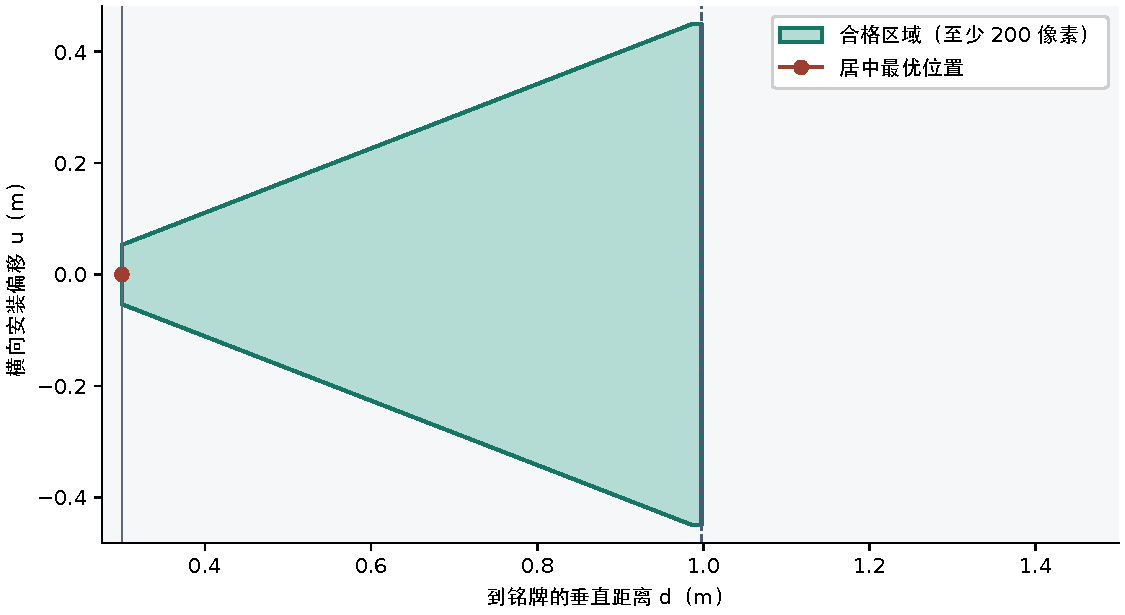
\includegraphics[width=.75\linewidth,height=.23\textheight,keepaspectratio]{label_region.pdf}
\caption{满足完整入镜和像宽要求的相机距离与横向偏移。}\label{fig:plate}
\end{figure}
\begin{table}[H]\centering
\caption{最低像宽对可行区域的影响。面积占比以夹具全部设置构成的 \(1.08\,\mathrm{m}^2\) 参数矩形为分母。}
\PlateTable
\end{table}
以投影像宽 \(P(d)\) 最大为目标。由于 \(P(d)\) 随 \(d\) 严格递减，当 \(d=0.30\) 时，凡满足 \(|u|\leq0.053205\) 的横向位置均为最优。取 \(u=0\) 居中放置，可以使左右两侧余量中较小的一侧也达到最大，两侧各余 147.45 像素。此时标称像宽为 665.11 像素。作为独立核验，在 \(9600\times6400\) 个网格单元的中点逐一投影铭牌的左右边缘；三个像宽门槛下，网格估计面积与积分结果的差均不超过 \(3.3\times10^{-5}\,\mathrm{m}^2\)。

\clearpage
\subsection{存在安装误差时的夹具设置}
理想条件下的最优解把相机设在允许的最近位置，安装时稍向铭牌靠近就会越过机械行程下限。设夹具的标称设置为 \((d_0,u_0)\)，实际位置可在 \(d_0\pm e,\ u_0\pm v\) 的范围内变化。这里的公差是算例设定，允许该矩形误差域内轴向和横向偏差的所有组合。

令 \(U=0.45\)、\(D=\min(1.50,960w/(2tP_0))\)。要使任何允许偏差下的实际位置均满足机械行程、左右边缘入镜和最低像宽要求，标称设置必须且只需满足
\begin{align}
 e+\max\{0.30,(w/2+v)/t\}\ \leq &\,d_0\leq D-e,\\
 |u_0|\ \leq &\,\min\{U-v,(d_0-e)t-w/2-v\}.
\end{align}
在最近位置 \(d_0-e\)，相机的水平视野最窄；在最远位置 \(d_0+e\)，铭牌所占的像素数最少。横向偏移绝对值最大可达 \(|u_0|+v\)。误差域包含四个角点，所以上述极端情况均可实际取到，据此得到的条件既充分又必要。这三个极值也决定了各标称距离下的可用横向宽度，沿标称距离积分即可得到可行面积。

\begin{table}[H]\centering
\caption{轴向与横向公差相等时，最优居中设置下可保证的成像指标。面积占比均以原始 \(1.08\,\mathrm{m}^2\) 参数矩形为分母。}
\ToleranceTable
\end{table}
要让最不利情况下的像宽尽可能大，应取最小可行的 \(d_0\)，再通过居中设置使余量较小的一侧获得最大的保证值。当 \(e=v=1\) cm 时，标称距离取 31\,cm，实际距离在 30 至 32\,cm 之间。铭牌至少占 623.54 像素，两侧中余量较小的一侧也至少留有 119.73 像素。与理想安装相比，可行面积占比由 32.89\% 降至 29.97\%。

在 \(4800\times3200\) 个标称位置构成的网格上，分别检查误差矩形四个角点处铭牌两端的投影。对每档公差，直接投影与解析式在每个受检网格点给出的可行性判断均一致。这项检验验证了几何计算。200 像素门槛规定的是取景和采样要求；要检验铭牌文字能否读清，还需使用文字内容已知的样本图像，并测量模糊程度和照明条件。

\clearpage
\section{问题二　测温通道选择与初始工单排程}
\subsection{两路测温通道的选择}
通道 A、B、C、D 的读数依次为 \(22.4,22.7,22.1,22.6^\circ\mathrm C\)，各自独立的重复性误差标准差依次为 \(0.35,0.45,0.60,0.90^\circ\mathrm C\)。准备一次读数分别耗用 \(8,7,4,2\) 仪器分钟。记 \(Y_i=T+B+e_i\)，其中 \(T\) 为共同待测温度，参考偏差 \(B\) 的均值为零，标准差为 \(c=0.20^\circ\mathrm C\)。各 \(e_i\) 与 \(B\) 均为相互独立的高斯变量，且 \(\operatorname{Var}(e_i)=v_i\)。两路读数包含同一个 \(B\)。

选取通道 \(i,j\) 后，线性无偏估计量可写为 \(\hat T=w_iY_i+w_jY_j\)，其中 \(w_i+w_j=1\)。在此约束下最小化方差 \(c^2+w_i^2v_i+w_j^2v_j\)，得到最优权重与相应方差
\begin{equation}
 w_i=\frac{v_i^{-1}}{v_i^{-1}+v_j^{-1}},\qquad
 V_{ij}=c^2+\frac{1}{v_i^{-1}+v_j^{-1}} .
\end{equation}
该二次目标函数严格凸。无论如何选取权重，共有的参考偏差都会贡献 \(c^2\) 的方差。表~\ref{tab:pairs} 列出了全部通道组合，再根据准备时间筛选可行解。

\begin{table}[H]\centering
\caption{准备预算为 12 仪器分钟时的通道组合比较。}\label{tab:pairs}
\PairTable
\end{table}

可行组合中，A+C 的估计方差最小。两个通道的权重分别为 \(0.746114\) 和 \(0.253886\)，温度估计值为 \(22.32383^\circ\mathrm C\)。由已知误差方差可得 95\% 置信区间 \(\hat T\pm1.959964\sqrt{V_{AC}}=[21.61337,23.03430]^\circ\mathrm C\)。这个区间刻画了同一校准实验在给定条件下反复进行时，估计共同温度的不确定性。若参考仪器存在未知的固定偏差，则需要单独校准和修正。

预算为 10 仪器分钟时应选 A+D；预算增至 12 时，改用 C 替代 D；到 15 时，精度更高的 A+B 也满足预算。分别对六个组合的 \(2\times2\) 协方差矩阵直接求逆，可复现上述权重与估计方差。本节的通道编号与下文的工单编号相互独立。

\clearpage
\subsection{两个工位上的五张工单}
工单 \(j\) 先在一个检测工位处理 \(p_j\) 分钟，再由一名复核员用 \(q_j\) 分钟复核并签结。工单等候区容量不限。复核台按检测出件的顺序处理，每当工单就绪且工位空闲就立即开工。表~\ref{tab:jobs} 也列出了问题四中可能新增的工单。
\begin{table}[H]\centering
\caption{算例设定的各工序耗时。新增工单仅在相应场景中到达。}\label{tab:jobs}
\JobsTable
\end{table}
对排列 \(\pi\)，记其中第 \(i\) 张工单的检测和复核完工时刻分别为 \(I_i\) 和 \(C_i\)。取 \(I_0=C_0=0\)，可得递推关系
\[
 I_i=I_{i-1}+p_{\pi_i},\qquad
 C_i=\max(I_i,C_{i-1})+q_{\pi_i}.
\]
首要目标为最小化清空时刻 \(C_5\)。若多个排程并列，则先选择 \(\sum_i C_i\) 最小者，仍并列时按工单编号的字典序选择。对照策略采用初始登记顺序 A--B--C--D--E。
\begin{table}[H]\centering
\caption{登记顺序与最优顺序下的初始工单时间线，单位为分钟。}\label{tab:base}
\BaseTable
\end{table}
五张工单检测共需 34 分钟，末单复核至少还需 2 分钟，故 \(C_5\geq36\)。在 120 种排列中，B--C--D--A--E 等 8 种达到 36 分钟的下界，按登记顺序则需 39 分钟。先检测 B，复核台在第 3 分钟即可接单，B 的十分钟复核与 C 的检测可以并行。按 Johnson 两机排序规则，B--D--C--A--E 也在第 36 分钟清空\cite{johnson}。各单完工时刻之和在 Johnson 顺序下为 127 分钟，按本文并列规则可降至 124 分钟。

\clearpage
\subsection{测温准备占用检测工位时的联合决策}
前述 36 分钟对应五张工单的基本处理流程。现为工单 A 增加一项测温校验，假设所选两路通道的准备工作全程占用检测工位，两个通道依次准备，所需时间另加在 A 原有的十一分钟检测时间上。在此设定下，测温精度会影响其他工单共用的工位资源。问题四的停机比较仍采用基本处理时间。

若通道 \(i,j\) 各需准备 \(h_i,h_j\) 分钟，令 \(p_A'=11+h_i+h_j\)，其余处理时间保持不变。与前文相同，估计方差 \(V_{ij}\) 包含两路通道的共有参考方差。现同时最小化 \((C_{\max},\sqrt{V_{ij}})\)，找出其中的非支配组合：对于这些组合，若改选其他组合使一项指标更优，另一项指标就会变差。
\begin{figure}[H]\centering
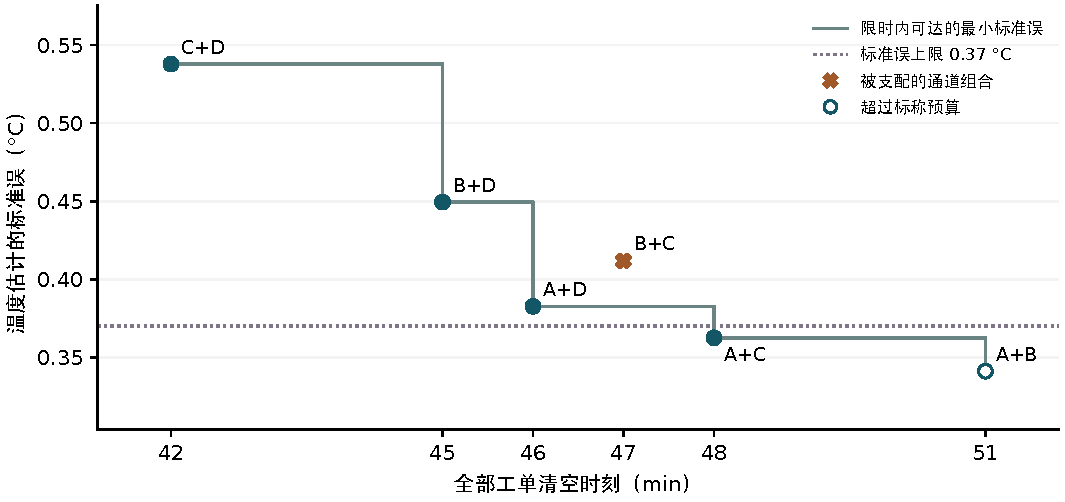
\includegraphics[width=.88\linewidth,height=.30\textheight,keepaspectratio]{joint_frontier.pdf}
\caption{测温标准误与全部五张工单最早清空时刻的关系。可选方案为离散的通道组合。}
\end{figure}
对六个通道组合分别评估全部 120 种工单顺序。对每个组合，B--C--D--A--E 都达到清空时刻下界 \(36+h_i+h_j\)，重新排列工单也无法消除新增的工位占用时间。在施加 12 仪器分钟的预算约束前，共有五个非支配组合。A+D 在两项指标上都优于 B+C：清空时刻从第 47 分钟提前至第 46 分钟，标准误从 \(0.412\) 降至 \(0.383^\circ\mathrm C\)。

在 12 仪器分钟预算内，要求第 46 分钟前（含该时刻）清空时应选 A+D；期限放宽至第 48 分钟，便可选 A+C，将标准误降至 \(0.362^\circ\mathrm C\)。若车间要求标准误不超过 \(0.37^\circ\mathrm C\)，最早可行的清空期限为第 48 分钟。额外耗时取决于通道准备是否实际占用检测工位，记录准备期间的工位占用情况即可判断应采用哪一版模型。

\clearpage
\section{问题三　固定参考标记的角度标定精度}
\subsection{圆周角误差的达标概率}
仪器观测一个位置已知、距离为 \(R=40\) 米的固定参考标记。累计移动距离达到 \(s\) 米后，两个坐标方向的误差相互独立，均服从 \(N(0,\sigma^2)\)，其中 \(\sigma=0.30+0.02s\)。仪器零偏误差和控制误差也相互独立，标准差分别为 \(0.8^\circ\) 和 \(0.6^\circ\)，合成标准差为 \(\tau=1^\circ\)。取三个相互独立的标准正态变量 \(X,Y,Z\)，总角误差可以写成
\begin{equation}
 D=\operatorname{wrap}_{[-\pi,\pi)}\!\left[
 \operatorname{atan2}(\sigma Y,R+\sigma X)+\tau Z\right].
\end{equation}
两个坐标误差的分布均关于零对称，因此交换其中任一误差分量的正负号约定不影响角误差的分布。令容差 \(\delta=5^\circ\)，要求达标概率 \(p(\sigma)=\Pr(|D|\leq\delta)\geq0.95\)。

给定 \(Z=z\)，将带坐标误差的参考向量旋转 \(g=\tau z\)，再除以 \(\sigma>0\)。由于坐标误差在平面内各向同性，该向量的协方差矩阵为单位阵，均值为 \((m,n)=(R/\sigma)(\cos g,\sin g)\)。设标准化后水平方向的残差为 \(u\)。对给定的 \(u\)，达标要求横坐标 \(m+u\) 为正，且纵坐标落在 \([-h,h]\) 内，其中 \(h=(m+u)\tan\delta\)。记标准正态分布的密度函数和分布函数为 \(\phi\) 和 \(\Phi\)，则
\begin{equation}
 p(\sigma)=\int_{\mathbb R}\!\phi(z)
 \int_{-m}^{\infty}\!\phi(u)
 \{\Phi(h-n)-\Phi(-h-n)\}\,du\,dz .
 \label{eq:sector}
\end{equation}
上述达标事件对应平面中的一个扇形，因此角度跨过 \(\pm\pi\) 的折返点时，判据仍然成立。

为证明临界值唯一，对不同 \(\sigma\) 使用同一组 \(X,Y\)。坐标误差引起的角偏差的绝对值为 \(\operatorname{atan2}(|Y|,R/\sigma+X)\)，几乎必然随 \(\sigma\) 严格增大。独立仪器误差服从以零为中心的卷绕正态分布。由文献~\cite{theta} 的 theta 函数乘积公式可知，其密度随到零点的圆周距离增大而严格递减。对于具有这一性质的偶密度 \(f\)，将半宽为 \(\delta\) 的弧段中心从零移至圆周距离 \(a\) 处时，弧内概率对 \(a\) 的导数为 \(f(a+\delta)-f(a-\delta)\leq0\)，两端点均按圆周角取值。由此可得 \(p(\sigma)\) 严格递减，方程 \(p(\sigma)=0.95\) 的根就是允许的最大坐标误差标准差。

\clearpage
\subsection{距离上限、独立模拟与方差贡献}
对式~\eqref{eq:sector} 采用 96 点高斯--勒让德求积，再求解 \(p=0.95\)，得到
\begin{equation}
 \sigma_* = 1.636745169\,\mathrm m,\qquad
 s_*=(\sigma_*-0.30)/0.02=66.83725843\,\mathrm m .
\end{equation}
若要求累计移动 80 米时依然达标，对误差模型 \(\sigma(s)=a+bs\)，其中 \(a,b\geq0\)，充要条件为 \(a+80b\leq\sigma_*\)。例如，保持 \(a=0.30\,\mathrm m\) 时，须有 \(b\leq(\sigma_*-0.30)/80\simeq0.016709315\)。标称参数给出 \(\sigma(80)=1.90\,\mathrm m\)，此时达标概率为 \(91.5068\%\)。

\begin{table}[H]\centering
\caption{积分结果与直接模拟结果。每个距离分别采用 200 万次独立试验。}\label{tab:noise}
\NoiseTable
\end{table}
\begin{figure}[H]\centering
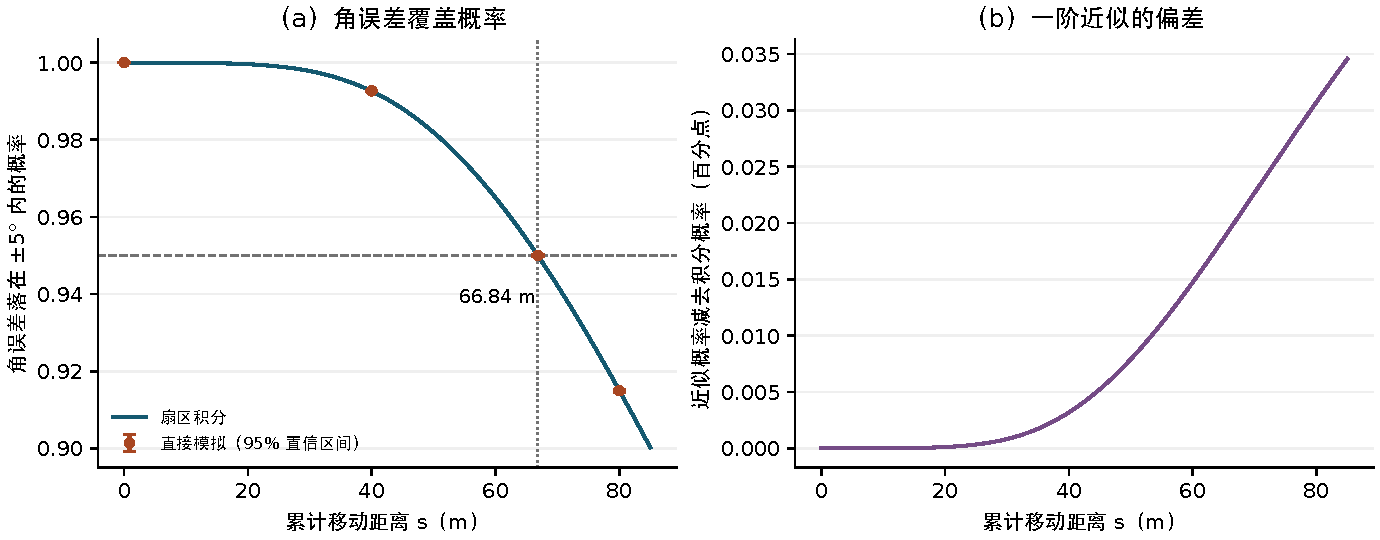
\includegraphics[width=.93\linewidth,height=.25\textheight,keepaspectratio]{q3_validation.pdf}
\caption{达标概率随累计移动距离的变化。右图单列一阶近似与积分结果之差。}\label{fig:noise}
\end{figure}
模拟分别对两个坐标误差分量以及零偏、控制两项仪器误差抽样。先用 \(\operatorname{atan2}\) 计算坐标偏差产生的角度，再加上仪器误差，将结果折回规定区间。表~\ref{tab:noise} 中的区间是各距离下分别计算的 95\% Wilson 置信区间~\cite{wilson}。不同距离共用同一组随机数，以减小距离间比较的抽样波动。将每个正态积分都截断在正负十个标准差内，舍去的概率不超过 \(4\Phi(-10)<3.1\times10^{-23}\)。改用 64 点或 128 点求积，所得 \(\sigma_*\) 与 96 点结果的差均小于 \(2\times10^{-13}\,\mathrm m\)。

在标称参考方向处作一阶线性化，角误差方差为 \(V_D\approx(\sigma/R)^2+\tau^2\)，单位为弧度平方。该近似给出的累计移动距离上限为 66.92230 米，比积分所得上限高 0.08504 米。在精确临界点处，按一阶模型分解总方差，坐标误差、零偏误差、控制误差分别占 84.61\%、9.85\% 和 5.54\%。若仅考察仪器误差，零偏和控制误差分别占其方差的 64\% 和 36\%。因此，在本算例的临界点附近，优先减小坐标漂移对降低总方差的一阶作用最大。

\clearpage
\section{问题四　扰动下的检修工单重排}
\subsection{第 8 分钟可以调整哪些工单}
两种策略都从队列 B--C--D--A--E 开始。第 8 分钟到达的通知给出新增工单及其工时，并在复核台停机时说明恢复时刻。此后不再发生其他扰动。此时 B 和 C 的检测都已开始，它们在队列中的位置固定。若停机打断了正在进行的复核，恢复后优先完成该单的剩余工作。恰好在第 36 分钟完成的工单计入按期完成数。

保留原序时，把新增工单依次追加到队尾。允许重排时，枚举尚未开始检测的工单的全部排列，原序也在其中。若改变顺序，需要在检测工位下一次空闲时占用它两分钟更新队列，在本例中为第 12 至 14 分钟。更新期间复核台可以继续工作。保留原序无需更新队列。

对每个可行顺序，程序按两道工序的递推关系计算时间线。若某单的复核跨过停机区间，则分别记录停机前后的两个工作时段。令 \(k=\#\{j:C_j\leq36\}\)，\(N\) 为截至通知时已公布的工单总数，含新增工单。先选取按期完成比例 \(k/N\) 较高的方案，比例相同再选实际清空时刻 \(C_{\max}\) 较早的方案。两项均相同时优先保留原序，此后按各单完工时刻之和最小、工单编号字典序择定代表解。另外记录以窗口终点封顶的末次完工时刻，只要有工单逾期，该指标即记为 36 分钟。实际清空时刻仍能区分封顶指标相同的逾期方案。
\begin{table}[H]\centering
\caption{相同扰动下的两种策略。按期完成数衡量截止前的交付量，实际清空时刻衡量全部工作结束的时间。}\label{tab:events}
\ScenarioTable
\end{table}
S0 为无扰动对照。S1 新增 F，S2 的复核台停机 8 分钟，S3 同时发生这两项扰动。S4 同时新增 F 和 G，S5 在此基础上再加 12 分钟停机。六个场景分别考察新增工作、产能暂时下降及二者的共同作用，不对各场景的发生概率作假设。

\clearpage
\subsection{重排在哪些场景下有收益}
\begin{figure}[H]\centering
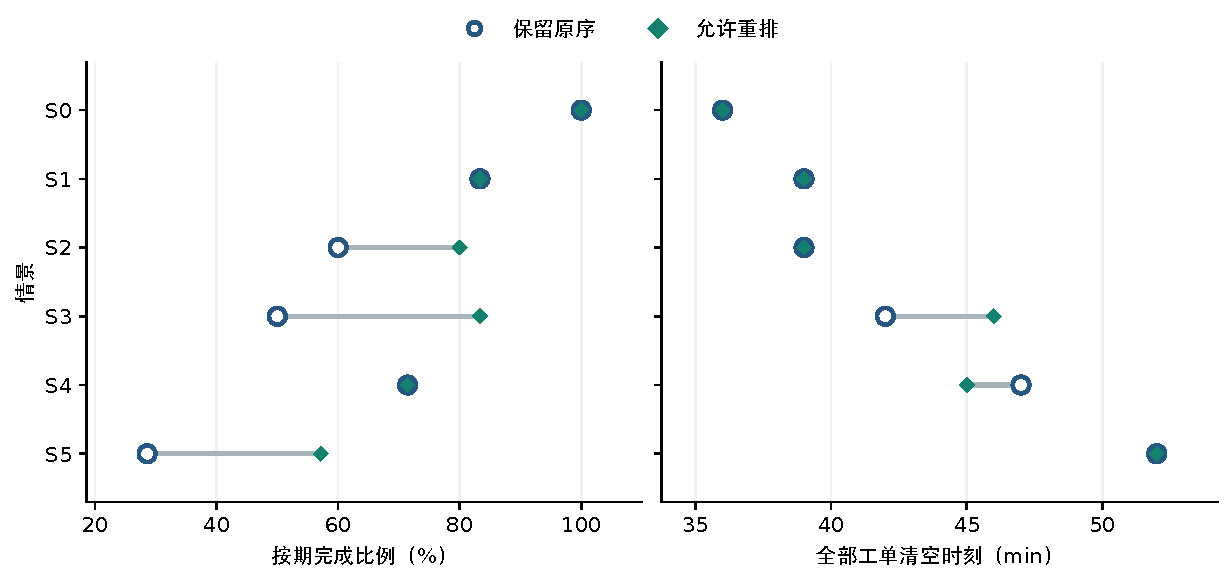
\includegraphics[width=.94\linewidth,height=.32\textheight,keepaspectratio]{schedule_comparison.pdf}
\caption{六个场景的策略比较。按期完成比例越高越好，实际清空时刻越早越好。}\label{fig:schedule}
\end{figure}
在 S0 和 S1 中，最优策略都保留原序。在 S2 中，将 E 提前可使按期完成数从 3 单增至 4 单，实际清空时刻不变。在 S3 中，将短工单 E 和 F 提前后，按期完成数从保留原序时的 3 单增至 5 单，实际清空时刻也从第 42 分钟推迟到第 46 分钟。若管理者更看重最后一单的完成时间，这一取舍就可能改变。

S4 体现了第二项评分指标的作用。两种策略都能按期完成 7 单中的 5 单，重排使清空时刻从第 47 分钟提前到第 45 分钟。在 S5 中，重排能按期完成 7 单中的 4 单，保留原序只能按期完成 2 单，两者均在第 52 分钟清空。允许重排的候选集包含按实际成本执行的原序，因此在本题规定的两级排序下，允许重排所得最优分数至少与保留原序相同。

\noindent\textbf{队列更新时间的敏感性。}\SensitivityText

\noindent\textbf{计算核验。}六个场景分别枚举 6、24、6、24、120、120 个候选后缀。对每个候选顺序，另以一分钟为步长回放过程，逐项核对剩余工时、工位占用和事件递推给出的各个区间。附录列出每个场景中两种策略的完整时间线。以上比较均以通知给出的恢复时刻准确为前提。

\clearpage
\subsection{在维修时长未知时决定队列}
现在设第 8 分钟时，车间知道新增了哪些工单，也知道复核台已停机，但必须在获知实际维修时长 \(L\) 前一次性选定剩余队列。已固定的前缀 B--C、两分钟队列更新时间、第 36 分钟截止和各工单工时保持不变。为考察提前获知维修时长的价值，令 4 至 16 分钟的 13 个整数时长等概率出现。该分布用于设定压力试验，未经现场故障数据拟合。

当 \(L=\ell\) 时，用 \(k(\pi,\ell)\) 表示队列 \(\pi\) 的按期完成数，\(C(\pi,\ell)\) 表示实际清空时刻。给定新增工单集合后，应对每个可能的时长采用同一个 \(\pi\)。若各时长的概率权重为 \(w_\ell\)，目标为
\[
 \mathop{\mathrm{lex\,min}}_{\pi}\left(
  -\sum_{\ell=4}^{16} w_\ell k(\pi,\ell),\
   \sum_{\ell=4}^{16} w_\ell C(\pi,\ell)\right).
\]
先最大化期望按期完成数，再从达到该最大值的队列中选取期望清空时刻最早的一组。比较的规则包括保留原序、将剩余工单按两道工序总工时从短到长排序、将平均维修时长代入模型求解，以及按上述双重期望目标求解。另设完全信息基准，允许对每个实际维修时长分别选取最优队列。各方法只要改变原序，均承担相同的队列更新开销。

\begin{table}[H]\centering
\caption{新增一张工单 F 时的策略比较。期望值按 13 个等概率维修时长计算。}
\RecoveryTable
\end{table}
新增 F 时，利用完整时长分布优化和代入平均维修时长得到相同的队列。若能提前知道实际维修时长，期望按期完成数仍然相同，但平均清空时刻可比预先选定队列提前 1.15 分钟。若只有复核台停机，没有新增工单，完整分布优化的期望按期完成数为 \(49/13=3.769\) 单，代入平均时长的结果为 \(48/13=3.692\) 单。即使已知各项工时的均值，直接代入均值仍可能错过最优队列。

\clearpage
\subsection{在哪些维修时长下值得重排}
\begin{figure}[H]\centering
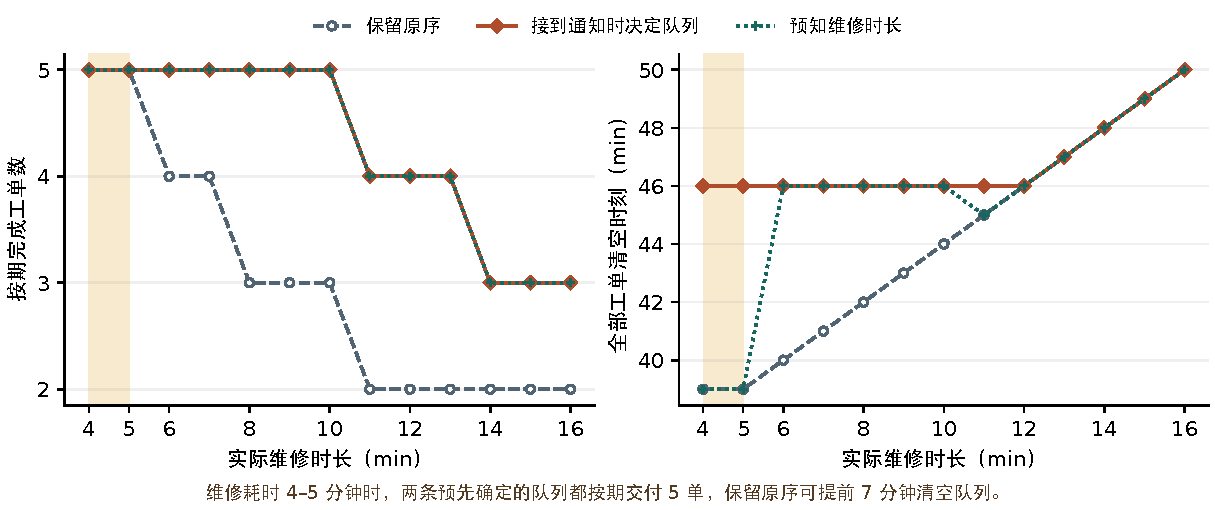
\includegraphics[width=.94\linewidth,height=.30\textheight,keepaspectratio]{uncertain_recovery.pdf}
\caption{新增工单 F。两条固定队列在通知时选定；完全信息基准可以预知维修时长。}\label{fig:repair}
\end{figure}
图~\ref{fig:repair} 中，若采用 B--C--E--F--A--D，维修耗时 8 至 13 分钟，重排恰好比保留原序多按期交付 2 单。这涵盖 13 个时长中的 6 个。如果维修仅用 4 或 5 分钟，两种队列都能按期完成 5 单，但原序在第 39 分钟清空，重排要到第 46 分钟。在其余 5 个时长下，重排比原序多按期交付 1 单。综合各时长，重排平均多按期交付 \(17/13=1.31\) 单，实际清空时刻平均推迟 \(35/13=2.69\) 分钟。

设每多按期交付一单，车间愿意让最后一单晚 \(v\ge0\) 分钟完成。在全部 24 条可行队列中最小化 \(\mathbb E[C]-v\mathbb E[k]\)。每条队列的成本都是 \(v\) 的一次函数。将 13 种维修时长的清空时刻与按期单数分别求和，可得到 13 倍成本的整数系数，由此得到表~\ref{tab:value} 的精确分界。
\begin{table}[H]\centering
\caption{新增 F、各维修时长等概率时的最低成本队列。在两个分界点，相邻两条队列并列最优。}\label{tab:value}
\small\begin{tabular}{@{}lcrr@{}}\toprule
可接受延迟 \(v\)（分钟/单）& 队列 & 期望按期单数 & 平均清空时刻（分钟）\\\midrule
\TradeoffRows
\bottomrule\end{tabular}
\end{table}
从原序 BCDAEF 改为 BCEFDA，平均多交付 \(12/13\) 单，只需多等 \(5/13\) 分钟，折合每单 \(5/12\) 分钟。再改为 BCEFAD，平均多交付 \(5/13\) 单，还需多等 \(30/13\) 分钟，折合每单 6 分钟。若只比较首尾两条队列，交点为 \(35/17\approx2.06\) 分钟/单；在这一位置，中间队列 BCEFDA 的成本严格更低。

对按期单数优先的目标，再按 \(17-\ell\) 和 \(\ell-3\) 为各维修时长赋予相对权重。平均维修时长分别为 8 和 12 分钟时，新增 F 的最优固定队列仍为 BCEFAD，期望按期单数分别为 4.70 和 3.91。三个到单情景共 \(13(6+24+120)=1950\) 个队列与时长组合，均经逐分钟回放核对。

\clearpage

\section{结论}
巡检方案取决于车间实际能够控制哪些条件。轴向和横向都允许 1\,cm 的安装公差时，相机的最优标称距离应调至 31\,cm。将清空期限从 46 分钟放宽到 48 分钟，便可把测温通道从 A+D 换为精度更高的 A+C。维修期间若新增一单，每多按期交付一单可接受的清空延迟在 \(5/12\) 至 6 分钟之间时，应把 E、F 提前，并把 D 排在 A 前。与保留原序相比，这条折中队列平均只晚 0.38 分钟清空，却平均多交付 0.92 单。

这些结论的适用范围由输入条件决定。在给定几何关系、高斯误差规律与工单工时后，数值计算和枚举可以复现上述决策。若要判断它们是否适用于真实车间，应重复测量夹具的实际位置，采集附有正确文字标注的铭牌照片，并记录带时间戳的工位占用与维修过程。再用后续班次的数据检验预测的容差命中率和工单完成情况，才能判断现场是否满足数值回放所依据的假设。

\begin{thebibliography}{9}
\bibitem{source} 数维杯组委会．2026 年秋季赛 B 题，第三问，第 4--5 页．本文角度标定参数的来源。
\bibitem{johnson} S. M. Johnson. Optimal two- and three-stage production schedules with setup times included. \emph{Naval Research Logistics Quarterly}, 1, 61--68, 1954. \url{https://doi.org/10.1002/nav.3800010110}.
\bibitem{theta} 美国国家标准与技术研究院（NIST）．\emph{Digital Library of Mathematical Functions}，第 20.5(i) 节，式 20.5.3，雅可比三重乘积公式．\url{https://dlmf.nist.gov/20.5.E3}。
\bibitem{wilson} NIST/SEMATECH．\emph{e-Handbook of Statistical Methods}，第 7.2.4.1 节，置信区间．\url{https://www.itl.nist.gov/div898/handbook/prc/section2/prc241.htm}。
\end{thebibliography}
\subsection*{计算与复现}
配套材料包含算例输入、六个数值计算脚本、计算结果、图表、表格生成程序和可编辑的论文源文件。OpenAI Codex 参与了练习数据的构造、计算和论文撰写。在主项目目录运行 \code{python reproduce.py} 可重新生成数值结果并编译英文修订稿；运行 \code{python reproduce.py --verify} 可校验文件哈希。中文解读文档列有运行环境和详细命令。中文版使用同一组数值结果，在中文版目录以 XeLaTeX 编译 \code{paper_zh.tex} 即可排版。

\clearpage
\section*{附录　工位时间线}
\addcontentsline{toc}{section}{附录　工位时间线}
下表均从初始工单发布时刻起算，单位为分钟。每一行给出一张工单在两种策略下经过检测工位和复核台的时间段。若复核区间分成两段，分别表示停机前与恢复后完成的工作。采用新顺序时，表中情景的检测工位均在 \([12,14)\) 分钟用于切换队列。各段之间的空档表示工位空闲或停用。
\AuditAppendix
\end{document}
